\documentclass[12pt]{article}
\usepackage[12pt]{moresize}

\usepackage{amsmath}
\usepackage{amssymb}

\usepackage{graphicx}
\usepackage{subcaption}

\usepackage{algorithm}
\usepackage{algpseudocode}
\usepackage{alltt}

\usepackage{multicol}

\usepackage[margin=1in]{geometry}

%\usepackage{hyperref}
%\usepackage[latin1]{inputenc}
%\usepackage{listings}
%\usepackage{scrextend}
%\usepackage{changepage} %Adjustwidth


\newenvironment{PTMono}{\fontfamily{PTMono-TLF}\selectfont}{\par}


\title{ComS 363\\Exam 2}
\author{Sean Gordon}
\date{April 6, 2020}

\begin{document}
\maketitle


\hrulefill \\[-.4em]



\noindent 1) \ (a) The records are fixed unpacked.\\
\indent (b) Page 1 and 3 would be unchanged, page 2's bitmap would be changed \\
\indent \indent from [1, 0, 1, 1, 0, 1] to [1, \textbf{1}, 1, 1, 0, 1] with the record added in the second slot.
\begin{figure}[h!]
  \centering
  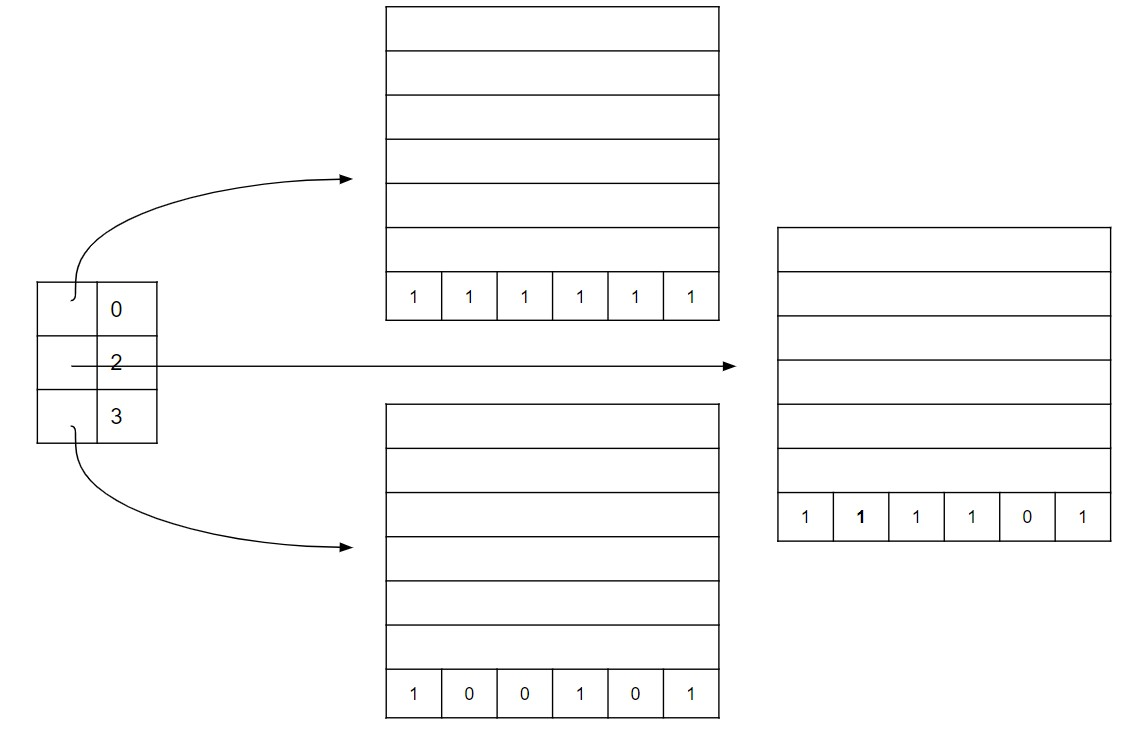
\includegraphics[scale=.6]{Exam2Q1.JPG}
\end{figure}\\
\indent (c) Because the records are unpacked, we need only reset the fourth bitmap slot in \\
\indent \indent page 2 to 0: [1, 0, 1, \textbf{0}, 0, 1].


\hrulefill\\


\noindent 2)\\
\indent Assuming 4 I/Os for traversal from root to leaves\\
\indent Question asks for \# read from disk, so output IO will not be considered\\
\indent Page space = Full page size - reserved space \\
\indent Tuples per page = (Page space) / (Record size) \\
\indent Entries per page = (Page space)  / (Data size) \\
\indent Assuming Page space = 4k B, Record size = 40 B, Data size = 20 B.\\\\
\indent (a) As the salaries are not indexed, each page must be searched to check for a match.\\
\indent \indent Thus, all 1000 pages must be read.\\
\indent (b) \# of matching pages for a sparse tree = 400 / (Tuples per page)\\
\indent \indent \# of pages of matching data entries = (\# of matching pages) / (\# Entries per page)\\
\indent \indent This results in (Traversal) + (\# Matching Pages) + (\# Pages of matching entries) = \\
\indent \indent 4 + 400 + 2 = 406 pages.
\indent (c) \# of matching entries for a dense tree = 400 / (Entries per page)\\
\indent \indent Total pages = (Traversal) + (\# of matching pages) + (\# Matching Entries) = \\
\indent \indent 4 + 400 + 2 = 406 pages.\\


\hrulefill\\\\


\noindent 3) \# of blocks of R = {\Large $\frac{M}{B-2}$}\\
\indent  Cost of join = M + ({\Large $\frac{M}{B-2}$}) * N.\\
\indent  \# of output pages = \# of blocks of R = {\Large $\frac{M}{B-2}$}\\
\indent  Thus total cost = M + ({\Large $\frac{M}{B-2}$}) * N + ({\Large $\frac{M}{B-2}$})\\\\


\hrulefill\\\\


\noindent 4) \\[.4em]
\textbf{Partition:} In this phase, we partition S using a hash function to put its tuples into output buffers, writing them to disk as needed. Afterward, we partition R using a hash function to put its tuples into output buffers, writing them to disk as needed. We have now divided all keys into different partitions.\\

\noindent \textbf{Join:} Read a page of R from partition x and construct a hash table of it., then read a page of S from partition x and probe the hash table for matches, concatenating them and putting them into the output buffer, flushing output to disk as necessary.\\\\


\hrulefill\\


\noindent 5) Out of the total memory, we need one page for an input buffer and one page for an output buffer, leaving us with one page to hold blocks of R. \\
\begin{algorithm}[H]
\caption{Grace hash join}
\begin{algorithmic} [1]
\ForAll{Tuple r in R}
\State bucketNum = H1(r) //Find which bucket r belongs to by using the hash function
\State Buckets[bucketNum].add(r)
\EndFor
\State 
\ForAll{Tuple s in S}
\State bucketNum = H1(s) //Find which bucket s belongs to by using the hash function
\State Buckets[bucketNum].add(s)
\EndFor
\State 
\ForAll{Bucket b in Table}
\State Use hash function H2 to build a new hash table
\State 
\ForAll{Page of r in b}
\ForAll{Tuple s in b}
\State Probe for any matches for s in page r
\State Store any matches in the output buffer, flush to disk if full
\EndFor
\EndFor
\State 
\EndFor

\end{algorithmic}
\end{algorithm}


\hrulefill\\



\noindent 6) \\
\indent (a) {\large $\pi_{sname}$($\sigma_{cid=="COMS363"}$(Register $\bowtie$ Students)) }\\[.4em]
\indent (b) {\large $\pi_{sname}$($\sigma_{semester=="Spring2020"}$(Register $\bowtie$ Students)) }\\[.4em]
\indent (b) {\large $\pi_{sname}$(Students) - $\pi_{sname}$(Register $\bowtie$ Students) }\\[.4em]


\hrulefill\\
\pagebreak


\noindent 7)\\
\begin{figure}[h!]
  \centering
  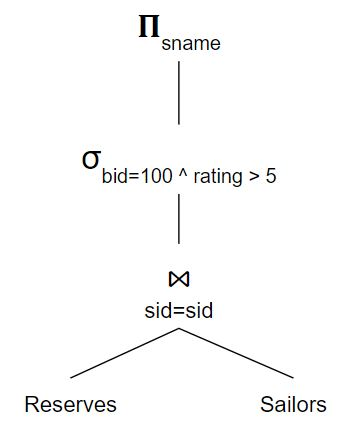
\includegraphics[scale=.6]{Exam2Q7.JPG}
\end{figure}


\hrulefill\\


\noindent 8)\\
\indent (a) Using left deep trees allows us to generate fully pipelined plans, meaning we can start from the bottom of the tree and work straight upward, without storing results temporarily. Everything is neatly funneled into a single `pipe'.\\

\indent (b) Because A $\bowtie$ B has the fewest I/Os, it will be performed, leaving the result to be merged with C and D in arbitrary order.\\
\begin{figure}[h!]
  \centering
  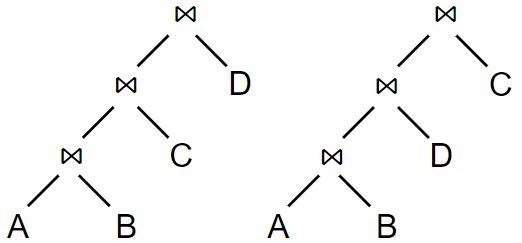
\includegraphics[scale=.6]{Exam2Q8b.JPG}
\end{figure}






\end{document}
















